% Options for packages loaded elsewhere
\PassOptionsToPackage{unicode}{hyperref}
\PassOptionsToPackage{hyphens}{url}
%
\documentclass[
]{article}
\usepackage{amsmath,amssymb}
\usepackage{iftex}
\ifPDFTeX
  \usepackage[T1]{fontenc}
  \usepackage[utf8]{inputenc}
  \usepackage{textcomp} % provide euro and other symbols
\else % if luatex or xetex
  \usepackage{unicode-math} % this also loads fontspec
  \defaultfontfeatures{Scale=MatchLowercase}
  \defaultfontfeatures[\rmfamily]{Ligatures=TeX,Scale=1}
\fi
\usepackage{lmodern}
\ifPDFTeX\else
  % xetex/luatex font selection
\fi
% Use upquote if available, for straight quotes in verbatim environments
\IfFileExists{upquote.sty}{\usepackage{upquote}}{}
\IfFileExists{microtype.sty}{% use microtype if available
  \usepackage[]{microtype}
  \UseMicrotypeSet[protrusion]{basicmath} % disable protrusion for tt fonts
}{}
\makeatletter
\@ifundefined{KOMAClassName}{% if non-KOMA class
  \IfFileExists{parskip.sty}{%
    \usepackage{parskip}
  }{% else
    \setlength{\parindent}{0pt}
    \setlength{\parskip}{6pt plus 2pt minus 1pt}}
}{% if KOMA class
  \KOMAoptions{parskip=half}}
\makeatother
\usepackage{xcolor}
\usepackage[margin=1in]{geometry}
\usepackage{color}
\usepackage{fancyvrb}
\newcommand{\VerbBar}{|}
\newcommand{\VERB}{\Verb[commandchars=\\\{\}]}
\DefineVerbatimEnvironment{Highlighting}{Verbatim}{commandchars=\\\{\}}
% Add ',fontsize=\small' for more characters per line
\usepackage{framed}
\definecolor{shadecolor}{RGB}{248,248,248}
\newenvironment{Shaded}{\begin{snugshade}}{\end{snugshade}}
\newcommand{\AlertTok}[1]{\textcolor[rgb]{0.94,0.16,0.16}{#1}}
\newcommand{\AnnotationTok}[1]{\textcolor[rgb]{0.56,0.35,0.01}{\textbf{\textit{#1}}}}
\newcommand{\AttributeTok}[1]{\textcolor[rgb]{0.13,0.29,0.53}{#1}}
\newcommand{\BaseNTok}[1]{\textcolor[rgb]{0.00,0.00,0.81}{#1}}
\newcommand{\BuiltInTok}[1]{#1}
\newcommand{\CharTok}[1]{\textcolor[rgb]{0.31,0.60,0.02}{#1}}
\newcommand{\CommentTok}[1]{\textcolor[rgb]{0.56,0.35,0.01}{\textit{#1}}}
\newcommand{\CommentVarTok}[1]{\textcolor[rgb]{0.56,0.35,0.01}{\textbf{\textit{#1}}}}
\newcommand{\ConstantTok}[1]{\textcolor[rgb]{0.56,0.35,0.01}{#1}}
\newcommand{\ControlFlowTok}[1]{\textcolor[rgb]{0.13,0.29,0.53}{\textbf{#1}}}
\newcommand{\DataTypeTok}[1]{\textcolor[rgb]{0.13,0.29,0.53}{#1}}
\newcommand{\DecValTok}[1]{\textcolor[rgb]{0.00,0.00,0.81}{#1}}
\newcommand{\DocumentationTok}[1]{\textcolor[rgb]{0.56,0.35,0.01}{\textbf{\textit{#1}}}}
\newcommand{\ErrorTok}[1]{\textcolor[rgb]{0.64,0.00,0.00}{\textbf{#1}}}
\newcommand{\ExtensionTok}[1]{#1}
\newcommand{\FloatTok}[1]{\textcolor[rgb]{0.00,0.00,0.81}{#1}}
\newcommand{\FunctionTok}[1]{\textcolor[rgb]{0.13,0.29,0.53}{\textbf{#1}}}
\newcommand{\ImportTok}[1]{#1}
\newcommand{\InformationTok}[1]{\textcolor[rgb]{0.56,0.35,0.01}{\textbf{\textit{#1}}}}
\newcommand{\KeywordTok}[1]{\textcolor[rgb]{0.13,0.29,0.53}{\textbf{#1}}}
\newcommand{\NormalTok}[1]{#1}
\newcommand{\OperatorTok}[1]{\textcolor[rgb]{0.81,0.36,0.00}{\textbf{#1}}}
\newcommand{\OtherTok}[1]{\textcolor[rgb]{0.56,0.35,0.01}{#1}}
\newcommand{\PreprocessorTok}[1]{\textcolor[rgb]{0.56,0.35,0.01}{\textit{#1}}}
\newcommand{\RegionMarkerTok}[1]{#1}
\newcommand{\SpecialCharTok}[1]{\textcolor[rgb]{0.81,0.36,0.00}{\textbf{#1}}}
\newcommand{\SpecialStringTok}[1]{\textcolor[rgb]{0.31,0.60,0.02}{#1}}
\newcommand{\StringTok}[1]{\textcolor[rgb]{0.31,0.60,0.02}{#1}}
\newcommand{\VariableTok}[1]{\textcolor[rgb]{0.00,0.00,0.00}{#1}}
\newcommand{\VerbatimStringTok}[1]{\textcolor[rgb]{0.31,0.60,0.02}{#1}}
\newcommand{\WarningTok}[1]{\textcolor[rgb]{0.56,0.35,0.01}{\textbf{\textit{#1}}}}
\usepackage{graphicx}
\makeatletter
\def\maxwidth{\ifdim\Gin@nat@width>\linewidth\linewidth\else\Gin@nat@width\fi}
\def\maxheight{\ifdim\Gin@nat@height>\textheight\textheight\else\Gin@nat@height\fi}
\makeatother
% Scale images if necessary, so that they will not overflow the page
% margins by default, and it is still possible to overwrite the defaults
% using explicit options in \includegraphics[width, height, ...]{}
\setkeys{Gin}{width=\maxwidth,height=\maxheight,keepaspectratio}
% Set default figure placement to htbp
\makeatletter
\def\fps@figure{htbp}
\makeatother
\setlength{\emergencystretch}{3em} % prevent overfull lines
\providecommand{\tightlist}{%
  \setlength{\itemsep}{0pt}\setlength{\parskip}{0pt}}
\setcounter{secnumdepth}{-\maxdimen} % remove section numbering
\newlength{\cslhangindent}
\setlength{\cslhangindent}{1.5em}
\newlength{\csllabelwidth}
\setlength{\csllabelwidth}{3em}
\newlength{\cslentryspacingunit} % times entry-spacing
\setlength{\cslentryspacingunit}{\parskip}
\newenvironment{CSLReferences}[2] % #1 hanging-ident, #2 entry spacing
 {% don't indent paragraphs
  \setlength{\parindent}{0pt}
  % turn on hanging indent if param 1 is 1
  \ifodd #1
  \let\oldpar\par
  \def\par{\hangindent=\cslhangindent\oldpar}
  \fi
  % set entry spacing
  \setlength{\parskip}{#2\cslentryspacingunit}
 }%
 {}
\usepackage{calc}
\newcommand{\CSLBlock}[1]{#1\hfill\break}
\newcommand{\CSLLeftMargin}[1]{\parbox[t]{\csllabelwidth}{#1}}
\newcommand{\CSLRightInline}[1]{\parbox[t]{\linewidth - \csllabelwidth}{#1}\break}
\newcommand{\CSLIndent}[1]{\hspace{\cslhangindent}#1}
\ifLuaTeX
  \usepackage{selnolig}  % disable illegal ligatures
\fi
\IfFileExists{bookmark.sty}{\usepackage{bookmark}}{\usepackage{hyperref}}
\IfFileExists{xurl.sty}{\usepackage{xurl}}{} % add URL line breaks if available
\urlstyle{same}
\hypersetup{
  pdftitle={Decision Analysis for Laser Leveling Application},
  pdfauthor={Marina, Sara, Kent, Frederic, Grace},
  hidelinks,
  pdfcreator={LaTeX via pandoc}}

\title{Decision Analysis for Laser Leveling Application}
\usepackage{etoolbox}
\makeatletter
\providecommand{\subtitle}[1]{% add subtitle to \maketitle
  \apptocmd{\@title}{\par {\large #1 \par}}{}{}
}
\makeatother
\subtitle{Creating a decision support model for smale scale farmers in
Vietnam using the decisionSupport R package by Lüdeling et al.}
\author{Marina, Sara, Kent, Frederic, Grace}
\date{2023-06-16}

\begin{document}
\maketitle

\begin{center}\rule{0.5\linewidth}{0.5pt}\end{center}

\hypertarget{introduction}{%
\section{Introduction}\label{introduction}}

\hypertarget{background}{%
\subsection{Background}\label{background}}

-Overview -potential benefits -relevance of the decision for farmers

\hypertarget{objective}{%
\subsection{Objective}\label{objective}}

-Determine whether laser leveling should be applied by a small farmer in
Vietnam

\hypertarget{methodology}{%
\section{Methodology}\label{methodology}}

-Methods we use -Decision analysis theory

\hypertarget{decision-criteria-maybe-with-data-sources}{%
\subsection{Decision Criteria (maybe with Data
Sources?)}\label{decision-criteria-maybe-with-data-sources}}

-features of our input table explained and sorted by overlying category
(eg. Economical, Ecological etc.)

\textbf{Economical Criteria} cost-effectiveness potential yield
improvement

\textbf{Ecological Criteria} environmental impact

\textbf{Social Criteria} ease of implementation

\hypertarget{package-management-section}{%
\subsection{Package Management
Section}\label{package-management-section}}

\begin{Shaded}
\begin{Highlighting}[]
\CommentTok{\# Install packages if needed (uncomment code):}
\CommentTok{\# install.packages("decisionSupport")}
\CommentTok{\# install.packages("dplyr")}
\CommentTok{\# install.packages("ggplot2")}

\FunctionTok{library}\NormalTok{(decisionSupport)}
\FunctionTok{library}\NormalTok{(dplyr)}
\end{Highlighting}
\end{Shaded}

\begin{verbatim}
## 
## Attaching package: 'dplyr'
\end{verbatim}

\begin{verbatim}
## The following objects are masked from 'package:stats':
## 
##     filter, lag
\end{verbatim}

\begin{verbatim}
## The following objects are masked from 'package:base':
## 
##     intersect, setdiff, setequal, union
\end{verbatim}

\begin{Shaded}
\begin{Highlighting}[]
\FunctionTok{library}\NormalTok{(ggplot2)}
\end{Highlighting}
\end{Shaded}

\hypertarget{data-preparation}{%
\section{Data Preparation}\label{data-preparation}}

\hypertarget{loading-and-organizing-existing-data-and-assumptions-made}{%
\subsection{Loading and organizing existing data and assumptions
made}\label{loading-and-organizing-existing-data-and-assumptions-made}}

\begin{Shaded}
\begin{Highlighting}[]
\CommentTok{\# data loading and sorting R code:}
\end{Highlighting}
\end{Shaded}

\hypertarget{analysis}{%
\section{Analysis}\label{analysis}}

\hypertarget{cost-benefit-analysis}{%
\subsection{Cost-benefit Analysis}\label{cost-benefit-analysis}}

A cost-benefit analysis comparing the expenses associated with laser
leveling to the potential benefits it may bring to the farmers was
conducted. The computations are done under the assumptions below.

\hypertarget{assumption-sources-for-4w-tractor-laser-leveler}{%
\subsubsection{Assumption sources for 4W tractor laser
leveler:}\label{assumption-sources-for-4w-tractor-laser-leveler}}

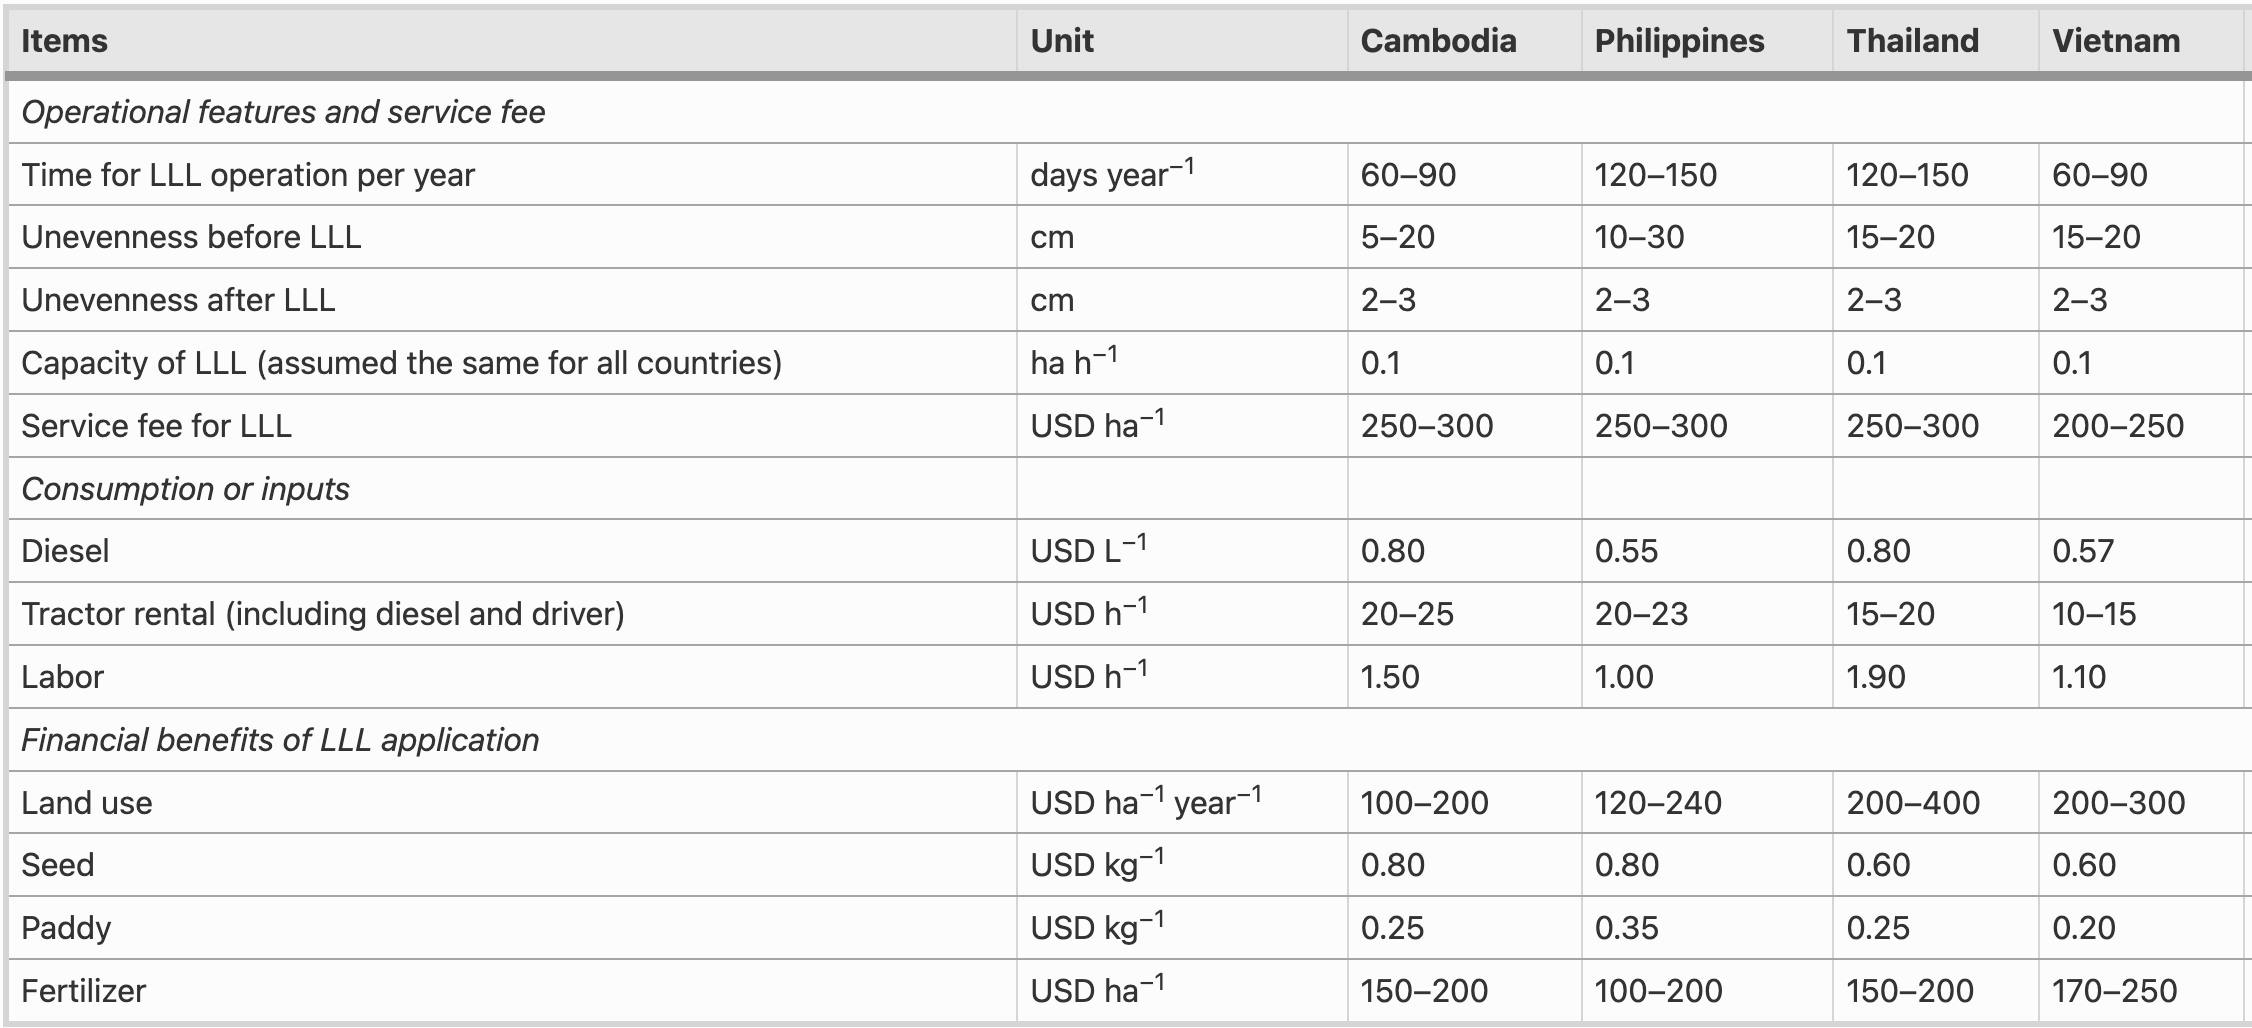
\includegraphics{images/Screenshot 2023-06-12 at 9.42.22 PM.png}

Source: (Nguyen-Van-Hung et al., 2022)

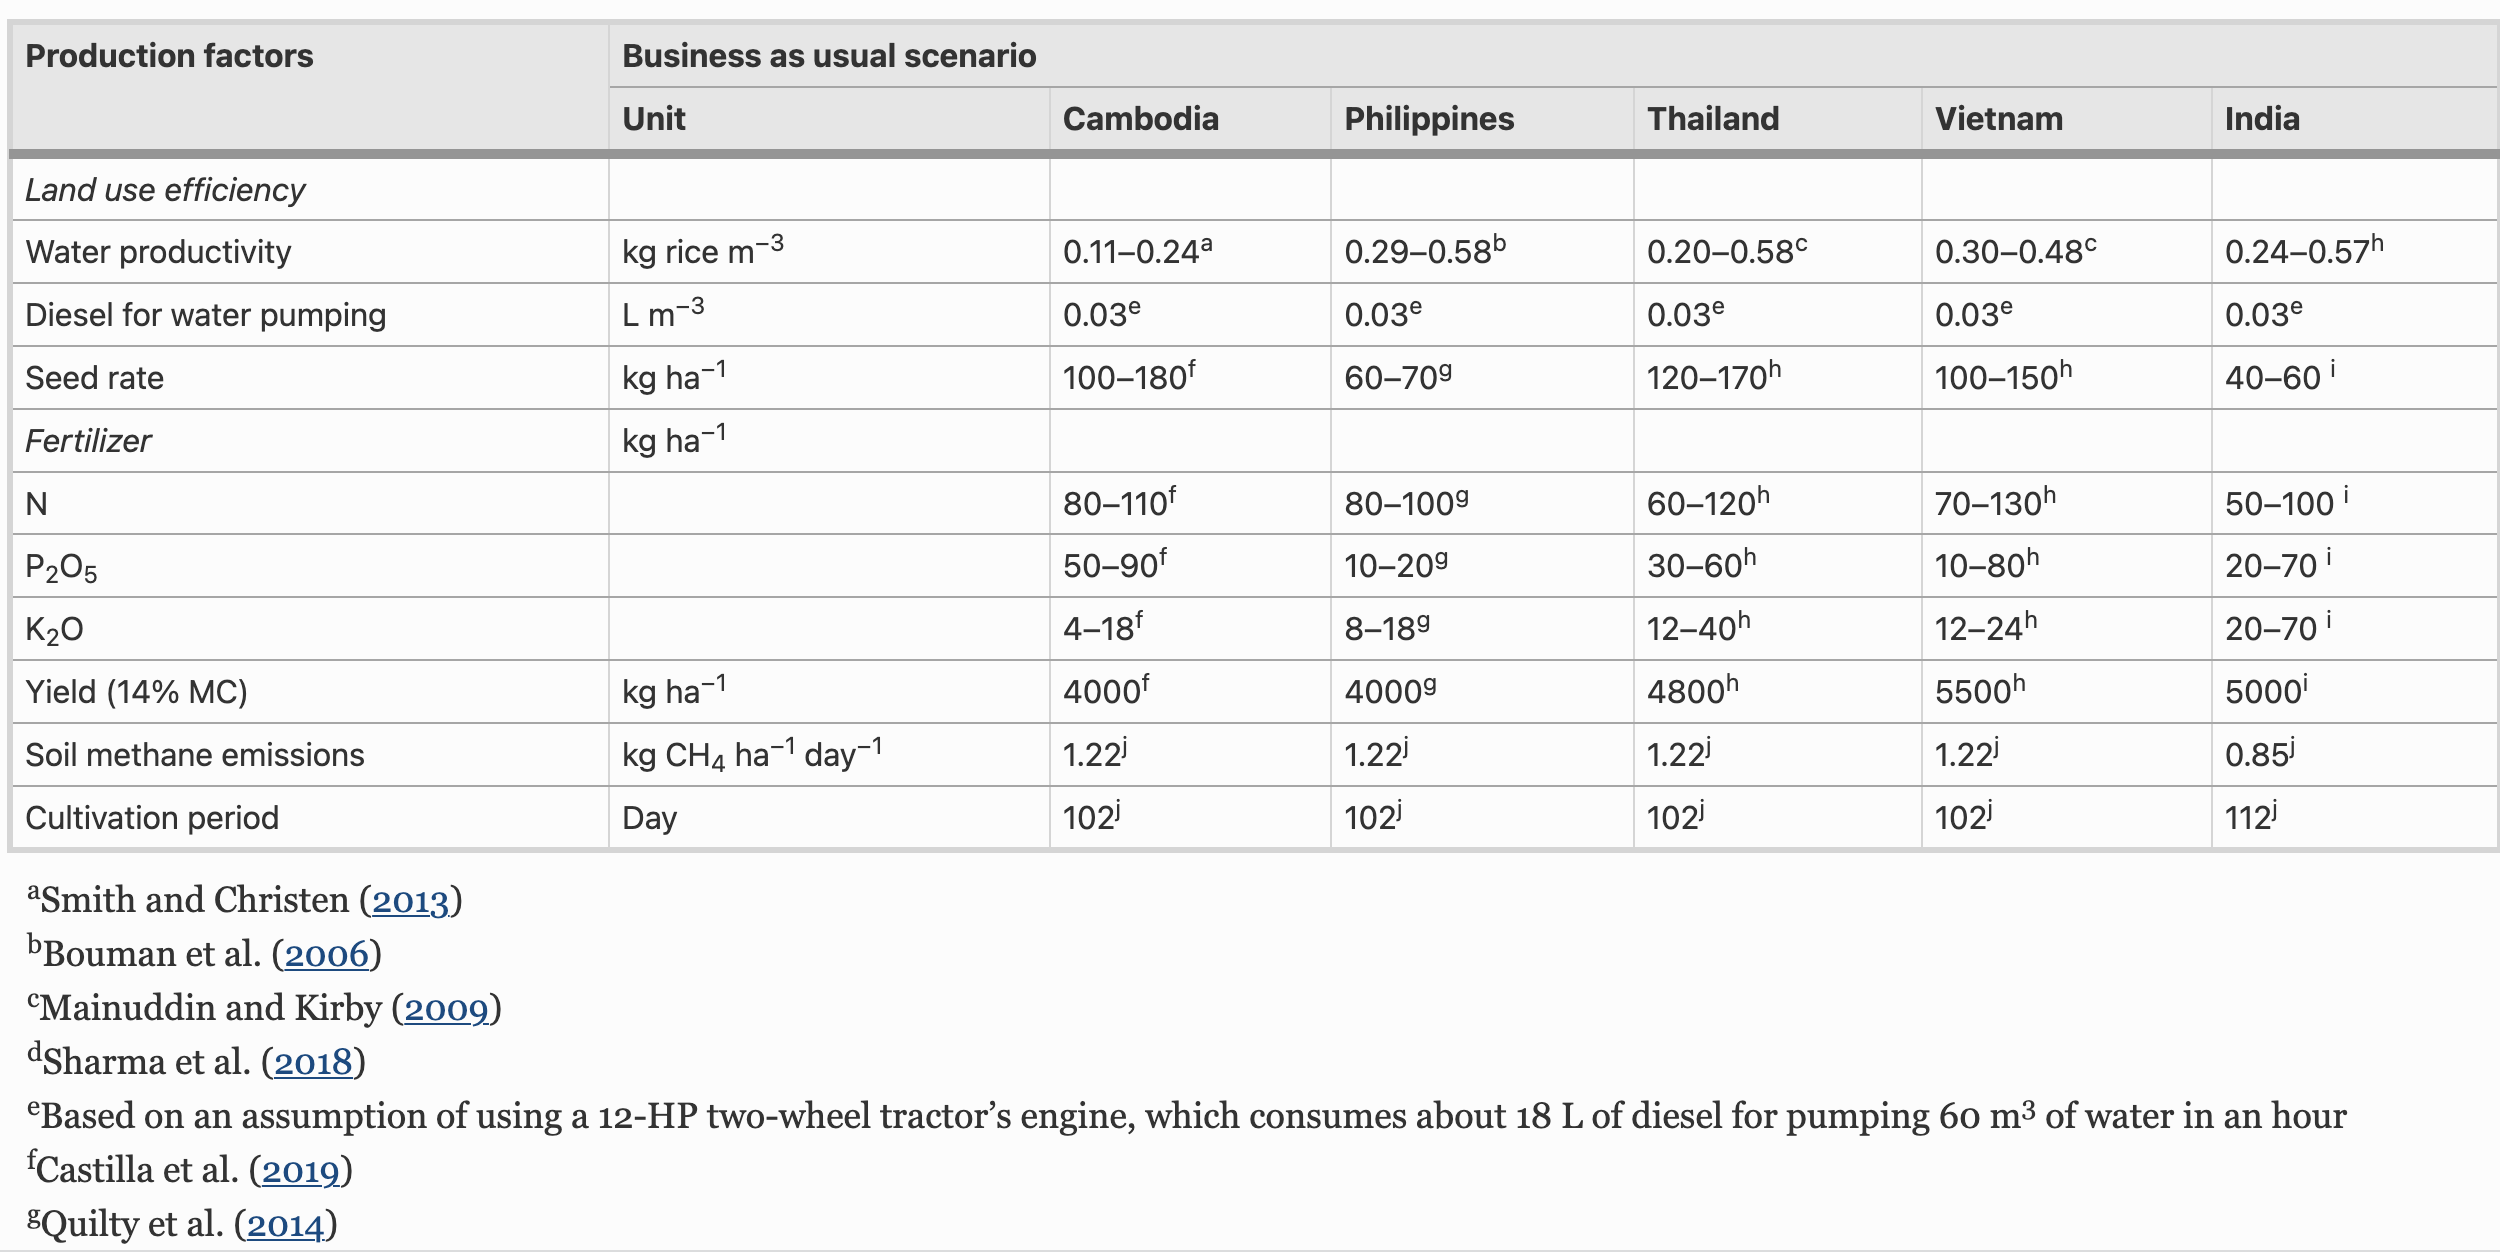
\includegraphics{images/Screenshot 2023-06-12 at 10.52.03 PM.png}

Source: (Nguyen-Van-Hung et al., 2022)

20000 VND-\textgreater{} minimum wage in Region II Vietnam (Dat, 2023)

7.8\% interest rate -\textgreater{} current rate for short term loans in
Vietnam (Worldbank, 2021)

40-50 USD/hr-\textgreater{} service fee for plowing

10 cropping seasons-\textgreater LLL will be done every 5 years, and
rice production will be done every cropping season

20\% additional input cost per season for re-smoothing of field

\hypertarget{code}{%
\subsubsection{Code}\label{code}}

\begin{Shaded}
\begin{Highlighting}[]
\FunctionTok{library}\NormalTok{(}\StringTok{"ggplot2"}\NormalTok{)}
\FunctionTok{library}\NormalTok{(dplyr)}
\CommentTok{\# cost analysis for LLL service provider (to be paid by farmer)}
\CommentTok{\#declaration of user input variables:}
\NormalTok{VND}\OtherTok{\textless{}{-}}\FloatTok{23487.50} \CommentTok{\#value of 1 USD to Vietnamese Dong (VND) as of date}
\DocumentationTok{\#\#\#operation (plowing, planting, harvest)}
\NormalTok{area\_covered}\OtherTok{\textless{}{-}} \DecValTok{3} \CommentTok{\#in ha}
\NormalTok{working\_days}\OtherTok{\textless{}{-}} \DecValTok{60} \CommentTok{\#in days}
\NormalTok{hours\_day}\OtherTok{\textless{}{-}}\DecValTok{8} \CommentTok{\#number of working hours per day}
\NormalTok{hrs\_area}\OtherTok{\textless{}{-}}\NormalTok{(area\_covered}\SpecialCharTok{/}\NormalTok{working\_days}\SpecialCharTok{/}\NormalTok{hours\_day)}\SpecialCharTok{*}\DecValTok{10000} \CommentTok{\#area to be covered in sq.m per hour}

\DocumentationTok{\#\#\#equipment sizing}
\NormalTok{speed\_op}\OtherTok{\textless{}{-}}\FloatTok{7.5} \CommentTok{\#speed of operation in km/hr}
\NormalTok{field\_ef}\OtherTok{\textless{}{-}}\DecValTok{40} \CommentTok{\#field efficiency in \%}
\NormalTok{LL\_size}\OtherTok{\textless{}{-}} \FloatTok{1.5} \CommentTok{\#commercially available size of drag bucket in m}
\NormalTok{actual\_area}\OtherTok{\textless{}{-}} \SpecialCharTok{+}\NormalTok{(LL\_size}\SpecialCharTok{*}\NormalTok{speed\_op)}\SpecialCharTok{*}\NormalTok{(field\_ef}\SpecialCharTok{/}\DecValTok{100}\NormalTok{)}\SpecialCharTok{*}\DecValTok{1000} \CommentTok{\#actual area covered in m2/hr}

\DocumentationTok{\#\#\#cost calculation}
\NormalTok{tractor\_price}\OtherTok{\textless{}{-}}\DecValTok{30000}\SpecialCharTok{*}\NormalTok{VND }\CommentTok{\#purchase price in Vietnamese Dong (VND)}
\NormalTok{usage\_tractor}\OtherTok{\textless{}{-}}\DecValTok{1200} \CommentTok{\#in hrs/yr}
\NormalTok{LL\_price}\OtherTok{\textless{}{-}}\DecValTok{12000}\SpecialCharTok{*}\NormalTok{VND }\CommentTok{\#purchase price of laser leveler in VND}
\NormalTok{usage\_LL}\OtherTok{\textless{}{-}} \SpecialCharTok{+}\NormalTok{working\_days}\SpecialCharTok{*}\NormalTok{hours\_day }\CommentTok{\#usage of laser leveler in hours/year}

\DocumentationTok{\#\#operating costs}
\NormalTok{engine\_power}\OtherTok{\textless{}{-}}\FloatTok{37.285} \CommentTok{\#in kW}

\NormalTok{fuel\_use}\OtherTok{\textless{}{-}}\SpecialCharTok{+}\NormalTok{engine\_power}\SpecialCharTok{/}\FloatTok{4.2} \CommentTok{\#in L}
\NormalTok{fuel\_cost}\OtherTok{\textless{}{-}}\FloatTok{22622.5} \CommentTok{\#in VND/L}
\NormalTok{fuel\_cost\_hr}\OtherTok{\textless{}{-}}\SpecialCharTok{+}\NormalTok{fuel\_cost}\SpecialCharTok{*}\NormalTok{fuel\_use }\CommentTok{\#fuel cost per hr}
\NormalTok{repair\_maintenance}\OtherTok{\textless{}{-}}\NormalTok{tractor\_price}\SpecialCharTok{/}\DecValTok{10}\SpecialCharTok{/}\NormalTok{usage\_tractor }\CommentTok{\#VND/hr}
\NormalTok{labor}\OtherTok{\textless{}{-}}\DecValTok{20000} \CommentTok{\#in VND/hr}
\NormalTok{total\_op\_cost}\OtherTok{\textless{}{-}}\SpecialCharTok{+}\NormalTok{repair\_maintenance}\SpecialCharTok{+}\NormalTok{fuel\_cost\_hr}\SpecialCharTok{+}\NormalTok{labor }\CommentTok{\#in VND/hr}

\DocumentationTok{\#\#fixed costs}
\NormalTok{tractor\_dep}\OtherTok{\textless{}{-}}\SpecialCharTok{+}\NormalTok{tractor\_price}\SpecialCharTok{/}\DecValTok{10}\SpecialCharTok{/}\NormalTok{usage\_tractor }\CommentTok{\#tractor depreciation in VND/hr}
\NormalTok{LL\_dep}\OtherTok{\textless{}{-}}\SpecialCharTok{+}\NormalTok{LL\_price}\SpecialCharTok{/}\DecValTok{10}\SpecialCharTok{/}\NormalTok{usage\_LL }\CommentTok{\#laser leveler depreciation in VND/hr}
\NormalTok{inv\_opp\_cost}\OtherTok{\textless{}{-}}\FloatTok{7.8} \CommentTok{\#investment/opportunity cost, a.k.a. interest for borrowing money}
\NormalTok{inv\_cost}\OtherTok{\textless{}{-}}\SpecialCharTok{+}\NormalTok{(tractor\_price}\SpecialCharTok{/}\NormalTok{usage\_tractor)}\SpecialCharTok{+}\NormalTok{((LL\_price}\SpecialCharTok{/}\NormalTok{usage\_LL)}\SpecialCharTok{*}\NormalTok{(inv\_opp\_cost}\SpecialCharTok{/}\DecValTok{100}\NormalTok{)) }\CommentTok{\#investment cost in VND/hr}
\NormalTok{total\_fixed\_cost}\OtherTok{\textless{}{-}}\NormalTok{tractor\_dep}\SpecialCharTok{+}\NormalTok{LL\_dep}\SpecialCharTok{+}\NormalTok{inv\_cost}

\NormalTok{total\_cost}\OtherTok{\textless{}{-}}\SpecialCharTok{+}\NormalTok{total\_op\_cost}\SpecialCharTok{+}\NormalTok{total\_fixed\_cost }\CommentTok{\#total cost in VND/hr}
\NormalTok{land\_lvl}\OtherTok{\textless{}{-}}\DecValTok{2} \CommentTok{\#average soil variation in cm}
\NormalTok{cost\_area}\OtherTok{\textless{}{-}}\NormalTok{total\_cost}\SpecialCharTok{/}\NormalTok{(actual\_area}\SpecialCharTok{/}\DecValTok{10000}\NormalTok{)}\SpecialCharTok{*}\NormalTok{land\_lvl }\CommentTok{\#cost/area in VND/ha}

\DocumentationTok{\#\#\#service provider}
\NormalTok{return\_mgt}\OtherTok{\textless{}{-}} \DecValTok{10} \CommentTok{\#return to management for operating the business in \%}
\NormalTok{service\_fee\_LLL}\OtherTok{\textless{}{-}}\NormalTok{(cost\_area}\SpecialCharTok{*}\NormalTok{((}\DecValTok{100}\SpecialCharTok{+}\NormalTok{return\_mgt)}\SpecialCharTok{/}\DecValTok{100}\NormalTok{))  }\CommentTok{\#in VND/ha, assuming LLL operation of 60 days per year}
\NormalTok{Input\_cost\_farmer}\OtherTok{\textless{}{-}}\NormalTok{service\_fee\_LLL}\SpecialCharTok{*}\NormalTok{(}\DecValTok{1}\FloatTok{+0.2}\SpecialCharTok{*}\DecValTok{9}\NormalTok{) }\CommentTok{\#in VND/ha under the assumption of LL operation every 5 years and resmoothing per season valued at 20\%}
\FunctionTok{print}\NormalTok{(Input\_cost\_farmer)}
\end{Highlighting}
\end{Shaded}

\begin{verbatim}
## [1] 14099185
\end{verbatim}

\begin{Shaded}
\begin{Highlighting}[]
\CommentTok{\#benefits for farmer}
\NormalTok{seed\_rate}\OtherTok{\textless{}{-}}\DecValTok{40} \CommentTok{\#kg/ha}
\NormalTok{yield}\OtherTok{\textless{}{-}}\DecValTok{5500} \CommentTok{\#at 14\% MC, kg/ha}
\NormalTok{N\_fert}\OtherTok{\textless{}{-}}\DecValTok{70} \CommentTok{\#kg/ha}
\NormalTok{P\_fert}\OtherTok{\textless{}{-}}\DecValTok{10} \CommentTok{\#kg/ha}
\NormalTok{K\_fert}\OtherTok{\textless{}{-}}\DecValTok{12} \CommentTok{\#kg/ha}
\NormalTok{land\_use}\OtherTok{\textless{}{-}}\DecValTok{200}\SpecialCharTok{*}\DecValTok{23487} \CommentTok{\#benefit in VND/ha/year}
\NormalTok{seed}\OtherTok{\textless{}{-}}\FloatTok{0.6}\SpecialCharTok{*}\DecValTok{23487} \CommentTok{\#benefit in VND/kg}
\NormalTok{paddy}\OtherTok{\textless{}{-}}\FloatTok{0.2}\SpecialCharTok{*}\DecValTok{23487} \CommentTok{\#benefit in VND/kg}
\NormalTok{fertilizer}\OtherTok{\textless{}{-}}\DecValTok{170}\SpecialCharTok{*}\DecValTok{23487} \CommentTok{\#benefit in VND/ha}
\NormalTok{season\_profit}\OtherTok{\textless{}{-}}\NormalTok{ ((land\_use)}\SpecialCharTok{/}\DecValTok{2}\NormalTok{)}\SpecialCharTok{+}\NormalTok{(seed}\SpecialCharTok{*}\NormalTok{seed\_rate)}\SpecialCharTok{+}\NormalTok{ (paddy}\SpecialCharTok{*}\NormalTok{seed\_rate) }\SpecialCharTok{+}\NormalTok{ (fertilizer)}\CommentTok{\#profit from season\textquotesingle{}s yields and savings after LLL in VND/ha}
\NormalTok{Output\_farmer}\OtherTok{\textless{}{-}}\NormalTok{ season\_profit }\SpecialCharTok{*}\DecValTok{10} \CommentTok{\#VND/ha for 10 cropping seasons}
\FunctionTok{print}\NormalTok{(Output\_farmer)}
\end{Highlighting}
\end{Shaded}

\begin{verbatim}
## [1] 70930740
\end{verbatim}

\begin{Shaded}
\begin{Highlighting}[]
\CommentTok{\#benefit{-}cost ratio}
\NormalTok{BC\_ratio}\OtherTok{\textless{}{-}}\NormalTok{ Output\_farmer}\SpecialCharTok{/}\NormalTok{Input\_cost\_farmer}
\FunctionTok{print}\NormalTok{(BC\_ratio)}
\end{Highlighting}
\end{Shaded}

\begin{verbatim}
## [1] 5.03084
\end{verbatim}

\begin{Shaded}
\begin{Highlighting}[]
\CommentTok{\#data visualization}
\NormalTok{cost\_shares}\OtherTok{\textless{}{-}}\FunctionTok{data.frame}\NormalTok{(}\AttributeTok{Portions=}\FunctionTok{c}\NormalTok{(}\StringTok{"Fuel consumption"}\NormalTok{,}\StringTok{"Repair and maintenance"}\NormalTok{,}\StringTok{"Labor cost"}\NormalTok{, }\StringTok{"Tractor depreciation"}\NormalTok{,}\StringTok{"Laser leveler depreciation"}\NormalTok{, }\StringTok{"Investment cost"}\NormalTok{), }\AttributeTok{share=}\FunctionTok{c}\NormalTok{(fuel\_cost\_hr, repair\_maintenance, labor, tractor\_dep, LL\_dep, inv\_cost))}


\NormalTok{cost\_shares }\OtherTok{\textless{}{-}}\NormalTok{ cost\_shares }\SpecialCharTok{\%\textgreater{}\%}
  \FunctionTok{arrange}\NormalTok{(}\FunctionTok{desc}\NormalTok{(Portions)) }\SpecialCharTok{\%\textgreater{}\%}
  \FunctionTok{mutate}\NormalTok{(}\AttributeTok{lab.ypos =} \FunctionTok{cumsum}\NormalTok{(share) }\SpecialCharTok{{-}} \FloatTok{0.5}\SpecialCharTok{*}\NormalTok{share)}

\NormalTok{mycols }\OtherTok{\textless{}{-}} \FunctionTok{c}\NormalTok{(}\StringTok{"\#0073C2FF"}\NormalTok{, }\StringTok{"\#EFC000FF"}\NormalTok{, }\StringTok{"\#868686FF"}\NormalTok{, }\StringTok{"\#CD534CFF"}\NormalTok{, }\StringTok{"\#00BA38"}\NormalTok{,}\StringTok{"\#A020F0"}\NormalTok{)}

\FunctionTok{ggplot}\NormalTok{(cost\_shares, }\FunctionTok{aes}\NormalTok{(}\AttributeTok{x =} \StringTok{""}\NormalTok{, }\AttributeTok{y =}\NormalTok{ share, }\AttributeTok{fill =}\NormalTok{ Portions)) }\SpecialCharTok{+}
  \FunctionTok{geom\_bar}\NormalTok{(}\AttributeTok{width =} \DecValTok{1}\NormalTok{, }\AttributeTok{stat =} \StringTok{"identity"}\NormalTok{, }\AttributeTok{color =} \StringTok{"white"}\NormalTok{) }\SpecialCharTok{+}
  \FunctionTok{coord\_polar}\NormalTok{(}\StringTok{"y"}\NormalTok{, }\AttributeTok{start =} \DecValTok{0}\NormalTok{)}\SpecialCharTok{+}
  \FunctionTok{geom\_text}\NormalTok{(}\FunctionTok{aes}\NormalTok{(}\AttributeTok{y =}\NormalTok{ lab.ypos, }\AttributeTok{label =}\StringTok{" "}\NormalTok{), }\AttributeTok{color =} \StringTok{"white"}\NormalTok{)}\SpecialCharTok{+}
  \FunctionTok{scale\_fill\_manual}\NormalTok{(}\AttributeTok{values =}\NormalTok{ mycols) }\SpecialCharTok{+}
  \FunctionTok{theme\_void}\NormalTok{()}
\end{Highlighting}
\end{Shaded}

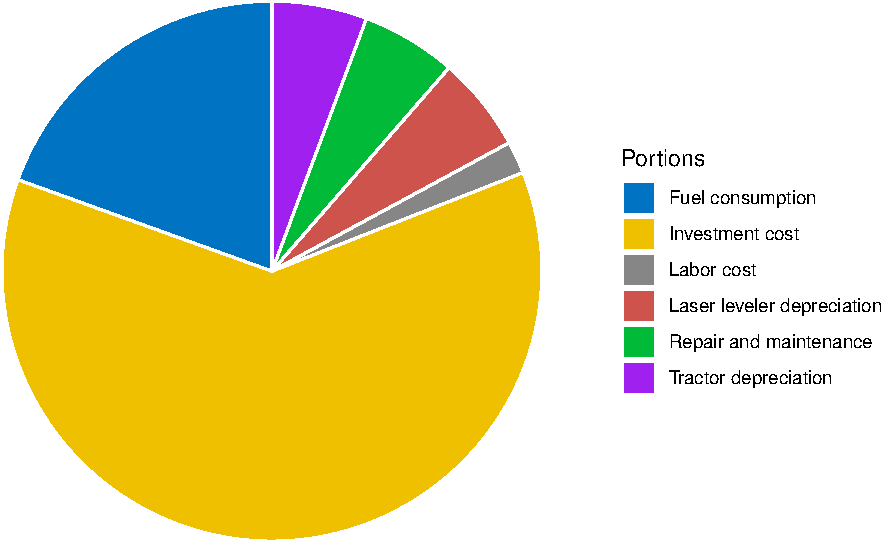
\includegraphics{Laser_leveling_simulation_files/figure-latex/cost-benefit-analysis-1.pdf}

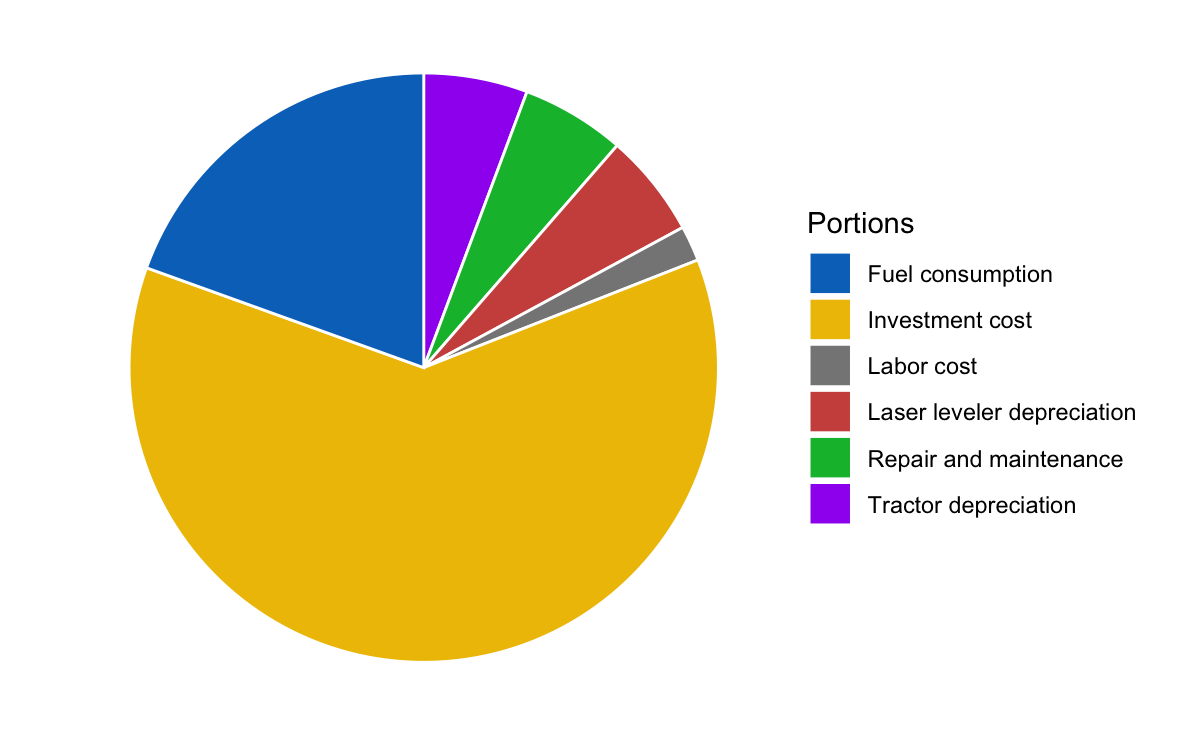
\includegraphics{images/Cost_portions.png}

Figure X. Cost proportions of LLL.

\hypertarget{yield-analysis}{%
\subsection{Yield Analysis}\label{yield-analysis}}

Performing an analysis to determine the potential yield improvement
laser leveling could offer in comparison to tradtional farming.

\hypertarget{assumption-sources}{%
\subsubsection{Assumption sources:}\label{assumption-sources}}

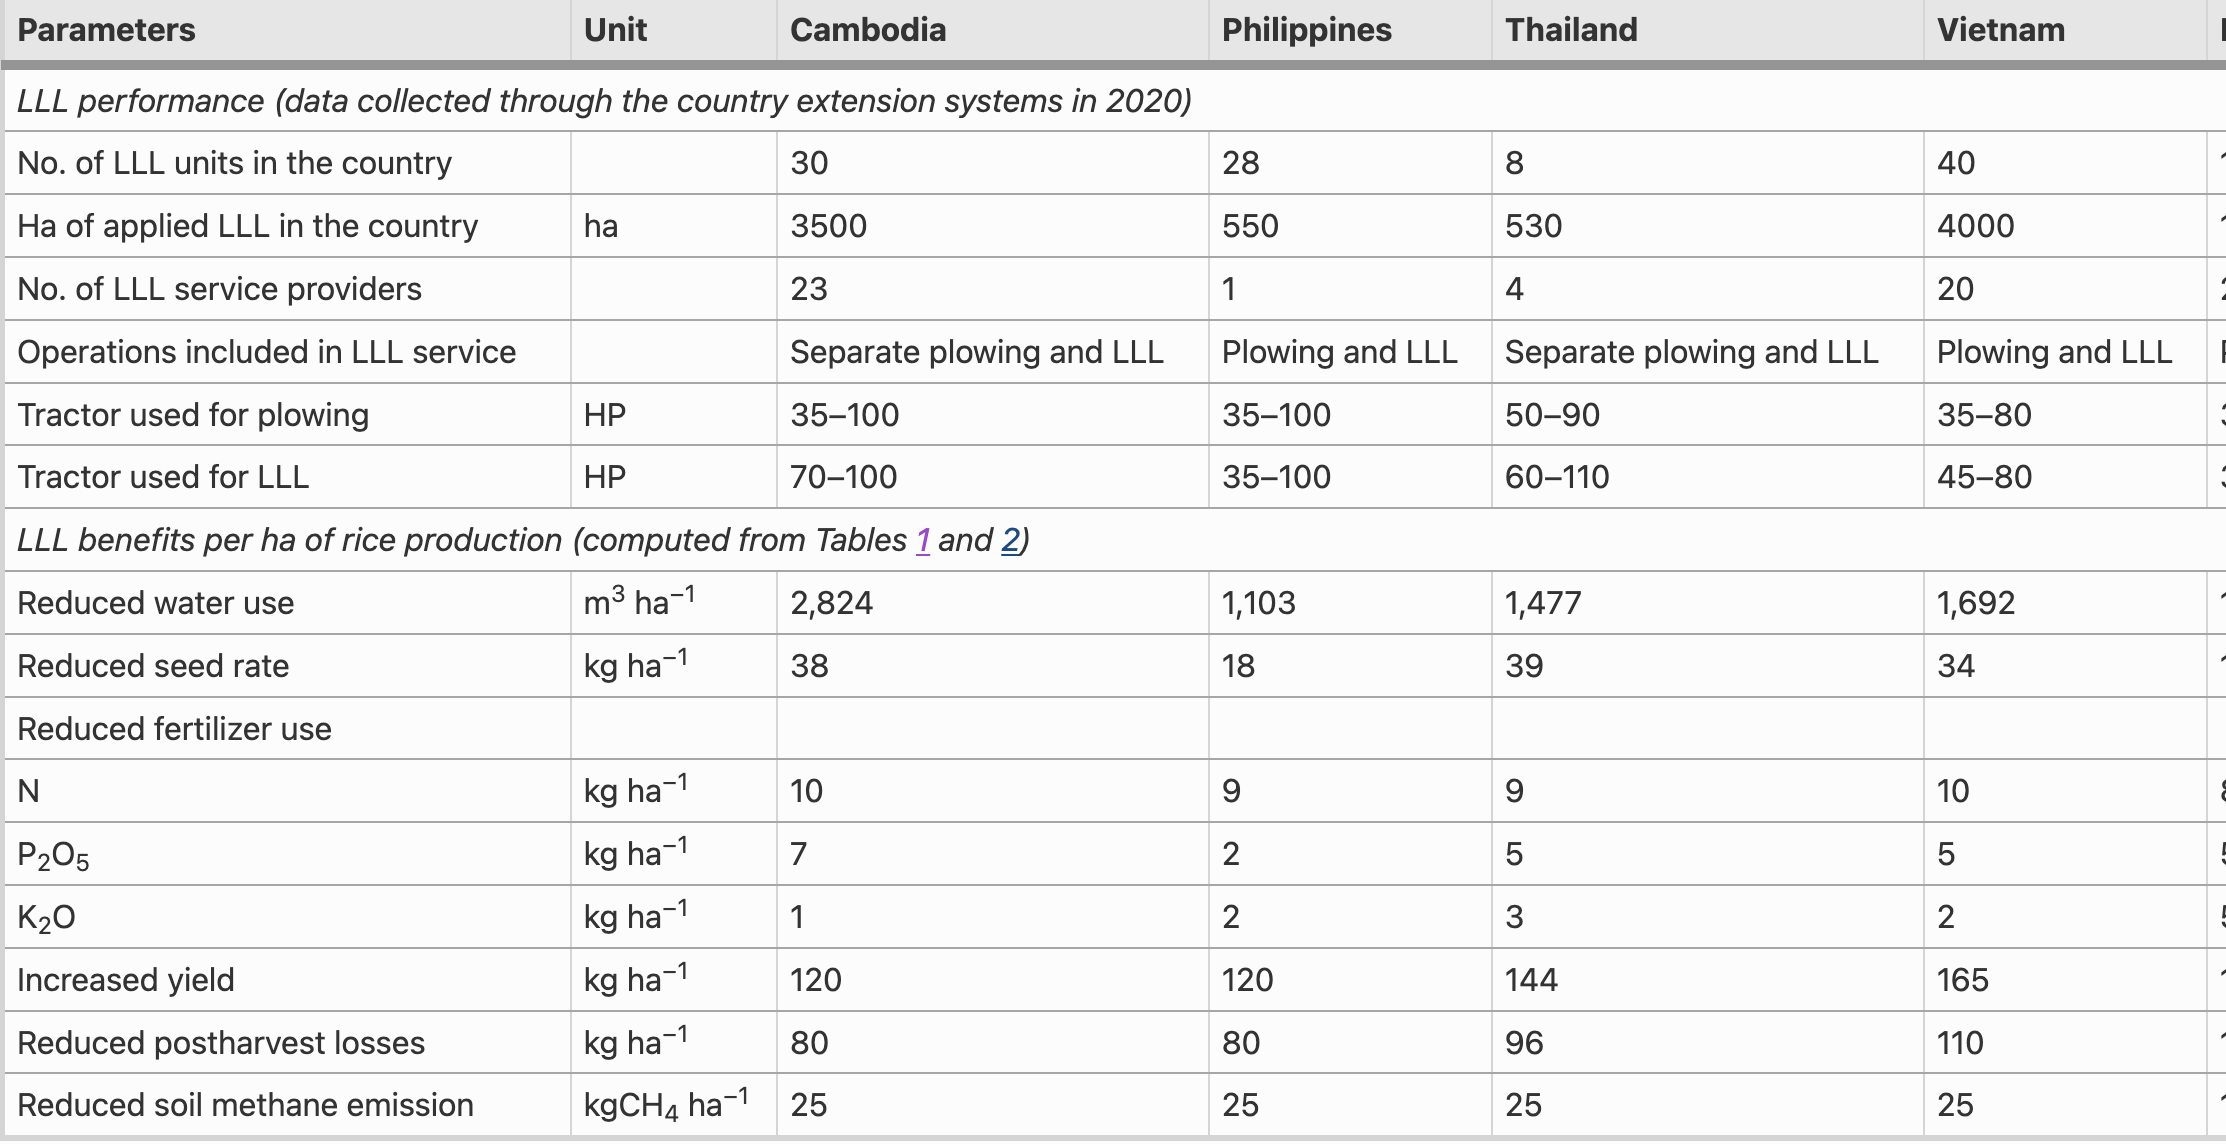
\includegraphics{images/Screenshot 2023-06-12 at 9.38.09 PM.png}

Source: (Nguyen-Van-Hung et al., 2022)

\begin{Shaded}
\begin{Highlighting}[]
\CommentTok{\# yield analysis R:}

\NormalTok{yield\_weight}\OtherTok{\textless{}{-}} \DecValTok{0} \CommentTok{\#weight of yield (total grains harvested in field at 14\% MC) in kg}
\NormalTok{field\_size}\OtherTok{\textless{}{-}}\DecValTok{0}  \CommentTok{\#typical field size in Vietnam in ha}
\NormalTok{GY}\OtherTok{\textless{}{-}}\NormalTok{ yield\_weight}\SpecialCharTok{/}\NormalTok{field\_size}
\end{Highlighting}
\end{Shaded}

\hypertarget{sensitivity-analysis}{%
\subsection{Sensitivity Analysis}\label{sensitivity-analysis}}

Conducting a sensitivity analysis to assess the impact of varying key
parameters and assumptions on the decision outcome. Maybe explore
different scenarios and evaluate their influence on the decision to
adopt laser leveling?

\begin{Shaded}
\begin{Highlighting}[]
\CommentTok{\# sensitivity analysis R code:}
\end{Highlighting}
\end{Shaded}

\hypertarget{results}{%
\section{Results}\label{results}}

\hypertarget{monte-carlo-simulation-results}{%
\subsection{Monte Carlo Simulation
Results}\label{monte-carlo-simulation-results}}

Include: -probability distributions -sensitivity analyses -relevant
metrics or charts that provide insights into the decision-making process

\begin{Shaded}
\begin{Highlighting}[]
\CommentTok{\# Monte Carlo simulation results R code:}
\end{Highlighting}
\end{Shaded}

\hypertarget{data-visualization}{%
\subsection{Data Visualization}\label{data-visualization}}

The simulated scenarios for the application of laser leveling visualized
using the \texttt{ggplot2} package (Wickham et al. 2023) -Time charts?

\begin{Shaded}
\begin{Highlighting}[]
\CommentTok{\# R code for vizualisation of results:}
\end{Highlighting}
\end{Shaded}

\hypertarget{decision-recommendation}{%
\subsection{Decision Recommendation}\label{decision-recommendation}}

-based on the analysis and simulation results of whether or not to
implement laser leveling considering: -decision criteria -cost-benefit
analysispotential risks and uncertainties.

\hypertarget{conclusion}{%
\section{Conclusion}\label{conclusion}}

-summary of the key findings -implications of the recommendation -areas
for future research or consideration

\hypertarget{references}{%
\section{References}\label{references}}

Dat, L. T. Q. (2023). What are monthly and hourly statutory minimum
wages in Vietnam? Retrieved from
\url{https://lawnet.vn/thong-tin-phap-luat/en/tu-van-luat/what-are-monthly-and-hourly-statutory-minimum-wages-in-vietnam-116511.html}

Nguyen-Van-Hung, Balingbing, C., Sandro, J. \emph{et al.} Precision land
leveling for sustainable rice production: case studies in Cambodia,
Thailand, Philippines, Vietnam, and India. \emph{Precision Agric}
\textbf{23}, 1633--1652 (2022).
\url{https://doi.org/10.1007/s11119-022-09900-8}

World Bank. (2021). Retrieved from
\url{https://data.worldbank.org/indicator/FR.INR.LEND?locations=VN}

\hypertarget{refs}{}
\begin{CSLReferences}{1}{0}
\leavevmode\vadjust pre{\hypertarget{ref-R-ggplot2}{}}%
Wickham, Hadley, Winston Chang, Lionel Henry, Thomas Lin Pedersen,
Kohske Takahashi, Claus Wilke, Kara Woo, Hiroaki Yutani, and Dewey
Dunnington. 2023. \emph{Ggplot2: Create Elegant Data Visualisations
Using the Grammar of Graphics}.
\url{https://CRAN.R-project.org/package=ggplot2}.

\end{CSLReferences}

\end{document}
